\begin{abstract}

Websockets have emerged as a leading technology in real-time communication systems. They allow for multi-duplex communication between systems.

Many companies have made a switch to microservice architectures. This presents some new challenges when integrating websockets into a microservice environment. Websockets are now speaking to different services behind the scenes. Developers need to know how their microservice environment reacts efficiently with minimal latency under certain loads when utilizing websockets. Many companies opt to use a PaaS (Platform as a service) to help them easily scale their applications. There are a number of PaaS systems on the market such as Pivotals Cloud Foundry, IBM Bluemix and GKE (Google Kubernetes Engine). These platforms expose powerful API's to gain insights into applications running on them.

The aim of this project is to create a websocket stress testing tool that can utilize Cloud Foundry's API in order to give developers a snapshot of how their entire microservice environment reacts under certain conditions.

\end{abstract}

\chapter{Research Context}
\lhead{\emph{Research Context}}

Websockets are a TCP based protocol\cite{8089962}. There have been a number of patterns and methods used in the past to simulate real-time communication. These include both polling and long polling. With polling, a client would make a request to a server continuously every few seconds. This method of communication had some drawbacks. It required connections to make a TCP handshake every time it reconnected. This handshake is costly as it takes a number of milliseconds to initiate. This is not a huge deal with just one connection. However when this is scaled up to hundreds of thousands of users then this TCP handshake will really impact a system\cite{5735801}. HTTP handshakes involve sending a SYN packet to the server which response with a SYN ACK to acknowledge the request then the client sends another SYN packet and connection is then established\ref{fig:http-handshake}\cite{5735801}. HTTP(s) further complicates the process as now the communication takes place over TLS (Transport Layer Security)\ref{fig:https-handshake}. 

\begin{figure}[ht]
  \centering
    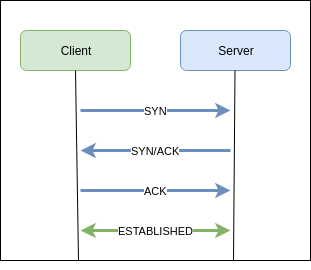
\includegraphics[width=0.5\textwidth]{figures/http-handshake.png}
    \caption{HTTP handshake}
    \label{fig:http-handshake}
\end{figure}

\begin{figure}[ht]
  \centering
    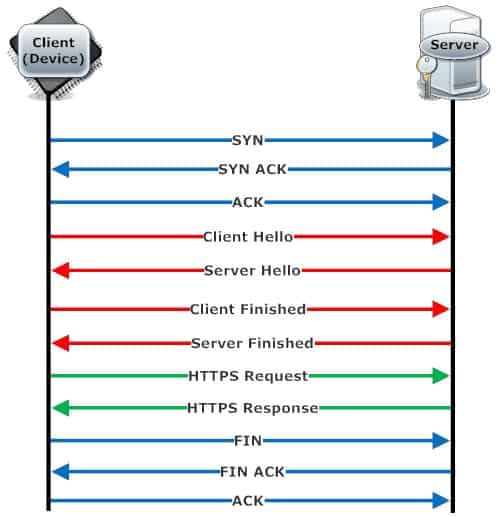
\includegraphics[width=0.5\textwidth]{figures/https-handshake.jpg}
    \caption{HTTP(s) handshake over TLS}
    \label{fig:https-handshake}
\end{figure}

Long polling tries to address this issue by making a request from the client to the server. The server then keeps the connection open for a specified amount of time. The server will wait for new information to arrive from somewhere. If data arrives before the connection times out then the connection is immediately terminated and the data is sent to the client. If no data has arrived by the time the connection times out then the connection is terminated and no data is sent to the client. In both cases the client will then reconnect and wait for more data to arrive. As specified in \cite{6364271}, long polling has one drawback in real time communication systems in that it needs more than one connection to achieve bi-directional communication.

There has been a huge shift from desktop devices to mobile devices\cite{6365155}. It has been proven that communication methods such as polling and long polling can have a negative affect on the batter life of mobile devices\cite{6364271}. This is due to the continuous connection and re-connection cycles, which are further exasperated by the fact that most of these connections are over cellular networks.

WebSockets aim to try and fix a lot of these shortcomings. This includes the ability to have full-duplex communication over a single persisted connection. WebSocket support is available in all major browsers, including mobile browsers. Once a connection is established between a server and a client, then both can communicate freely with each other by sending data encapsulated within a frame plus 2 extra bytes of payload, which is a huge reduction in payload from HTTP requests. There are 2 main stages to establishing and sending data over websockets. These include the handshake stage, which like polling and long polling is done over HTTP. The reason this is done over HTTP is because websocket protocols are built on top of HTTP. They also had backward compatibility in mind with HTTP in that you can send a GET request to a websocket server and the server will send back an UPGRADE request telling the client that communication over a websocket protocol is available. The client can then decide whether to upgrade or not.

\subsection{Resource Usage}

Websockets have been proven to require less system resources for real-time communication than polling and long polling. A study which done a comparative analysis of AJAX polling versus websockets found that polling increases the memory consumption over time compared to websockets which maintained a fairly constance memory consumption throughout\cite{6601579}. In terms of bandwidth usage when comparing polling versus websockets it was concluded that polling uses a larger amount of bandwidth over time, the reason for this was that polling required 256 bytes of extra data to be sent over the wire even if that 256 bytes of data is not used up, this means that in some cases there is can be a lot of white space sent over the network. The second reason was that the header data required for polling is significantly larger than that of a websockets header\cite{6601579}.

\subsection{Keep Alive Mechanisms}

Because WebSocket servers can hold potentially hundreds of thousands of connection open simultaneously, it is reasonable that the server may want to recycle some of these connections to prevent itself from becoming overloaded. Websockets support a keep alive mechanism to tell the server that the client is still actively using the connection. This is done in the form of a PING/PONG request. The server will send a ping request to the client, if the client is still active then it will respond with a pong. If the client does not respond then the server is free to terminate the connection and freeing up some resources in the process. 

\subsection{Websockets in a microservices environment}

Microservice architectures compliment websockets in a number of ways. In front of most microservice environments is an api gateway\cite{6885428}. This is a reverse proxy between a companies API layer and the the end user. It acts as security barrier preventing the user from having direct access to any of the underlying API's. Nginx is an example of a reverse proxy with websocket support. When a websocket connection is created Nginx will stream the websocket request onto the target service, then data will flow from the service through the gateway to the users client. 

While microservices do well to compliment websockets, there are sadly cases where a microservice can be difficult for websockets. Scaling applications is one such situation. Scaling means having multiple instances of the same service running at the same time with a load balancer in front which can chose the healthiest instance of a service to route requests to. Load balancing websockets can be a tricky task depending on how the websocket server is set up. The issue is that when you connect to a service, that connection is long lived, if there is a drop in connection and the websocket server re-connects then it is possible that the new connection may be connected to a different instance of the server the websocket was previously connected to. For this reason it is good practive to make websocket servers stateless. Best practictes suggest connecting the service to a backend queue such as RabbitMQ, Apache Kafka or Redis. This way of a websocket connection is dropped it will matter less which instance the reconnection request connects to.

\subsection{Microservice Monitoring}

Miroservice monitoring can be a daunting task\cite{7958458}. There are many widely used monitoring applications on the market such as Prometheous and Google CLoud Monitoring for Kubernetes environments. However to be able to get a snapshot of the system while automated tests are in progress with these tools would require a lot of user intervention such as filtering of dates and times on statistics for multiple running services. If the number of these services is high than this can be very time consuming. One of the goals of this project is to give a developer a snapshot of a system at a particular point in time, between the start of a websocket stress test and the end of the test.